%!TeX program = xelatex
\documentclass[xetex,aspectratio=169]{beamer}

\usepackage[spanish]{babel}
\usepackage{graphicx}
\usepackage{caption}
\usepackage{subcaption}

\usetheme{modern}


\title
    {Title}
\subtitle
    {Subtitle}
\author
    {Author}

\date{\today}

%\titlegraphic{
%    
\includegraphics[scale=0.05]{./imagotipos/usach_p1.png}
%}

%\logo{
%
\includegraphics[scale=0.04]{./imagotipos/usach_p1.png}
%}


\begin{document}
    
    
    \begin{frame}[plain, noframenumbering]
        \titlepage
    \end{frame}
    
    \begin{frame}{Table of contents}
        \begin{multicols}{2}
        	\tableofcontents[hideothersubsections]
        \end{multicols}
    \end{frame}
    
    %\section{Hello world}
    \section{Normal block}
    \begin{frame}{Frame in first section}
        \begin{block}{Normal block}
            Hello!        
        \end{block}

    \end{frame}
    
    \section{Alert block}
    \begin{frame}{Frame in second section}
        \begin{alertblock}{Alert Block}
            Alert!
        \end{alertblock}
    \end{frame}

    \section{Example block}
    \begin{frame}{Frame in third section}
        \begin{exampleblock}{Example Block}
            Example
        \end{exampleblock}
    \end{frame}

    \section{Itemize}
    \begin{frame}{Frame in fourth section}
        \begin{itemize}
            \item Item 1
            \item Item 2
            \item Item 3
        \end{itemize}
    \end{frame}

    \section{Enumerate}
    \begin{frame}{Frame in fourth section}
        \begin{enumerate}
            \item Item 1
            \item Item 2
            \item Item 3
        \end{enumerate}
    \end{frame}

    \section{Columns}
    \begin{frame}{Frame in fifth section}
        \begin{columns}
            \begin{column}{0.5\textwidth}
               Column 1 text
            \end{column}
            \begin{column}{0.5\textwidth}
                Column 2 text
            \end{column}
        \end{columns}    
    \end{frame}

    \section{Image}
    \begin{frame}{Frame in sixth section}
        \begin{figure}
            \centering
            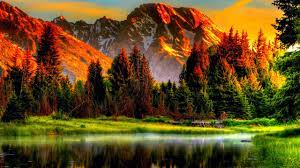
\includegraphics[width=0.5\textwidth, keepaspectratio]{example_images/nature1.jpg}
            \caption{Caption}
            \label{fig:enter-label}
        \end{figure}
    \end{frame}

    \section{Multiple images}
    \begin{frame}{Frame in seventh section}
        \begin{figure}
            \centering
            \begin{subfigure}{0.45\textwidth}
                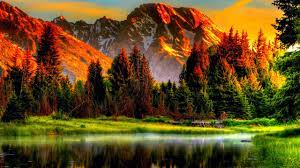
\includegraphics[width=.5\textwidth, keepaspectratio]{example_images/nature1.jpg} 
                \caption{Caption 1}
                \label{fig:subim1}
            \end{subfigure}
            %
            \begin{subfigure}{0.45\textwidth}
                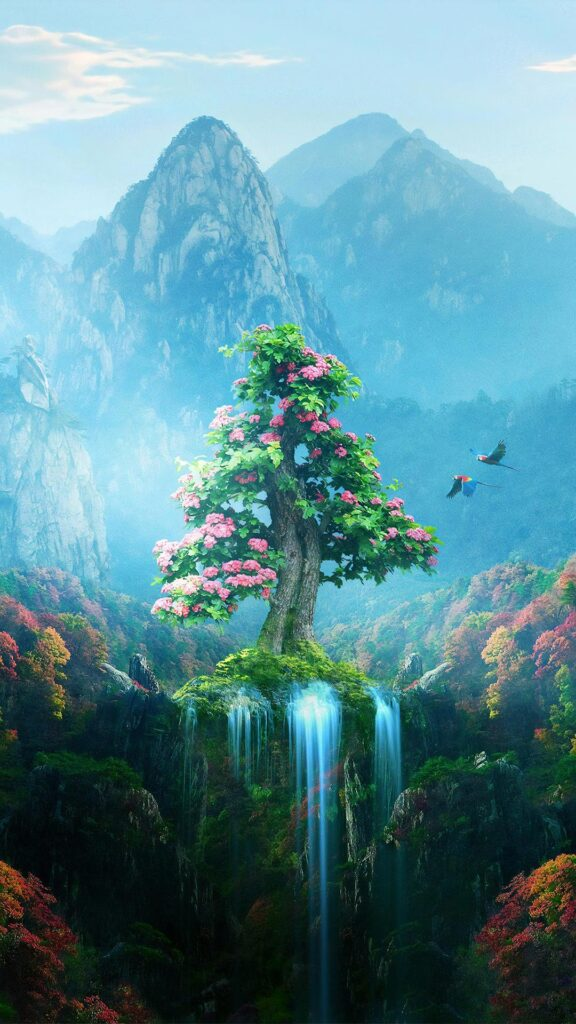
\includegraphics[width=.2\textwidth, keepaspectratio]{example_images/nature2-576x1024.jpg}
                \caption{Caption 2}
                \label{fig:subim2}
            \end{subfigure}
            
            \caption{Caption for this figure with two images}
            \label{fig:image2}
        \end{figure}
    \end{frame}

    \section{Overlap images}
    \begin{frame}{Frame in eighth section}
        \begin{center}
            % create a new tikz picture
            \begin{tikzpicture}
                \node (img1) {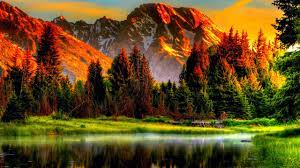
\includegraphics[height=3cm]{example_images/nature1.jpg}};
                \node (img2) at (img1.south east)
                {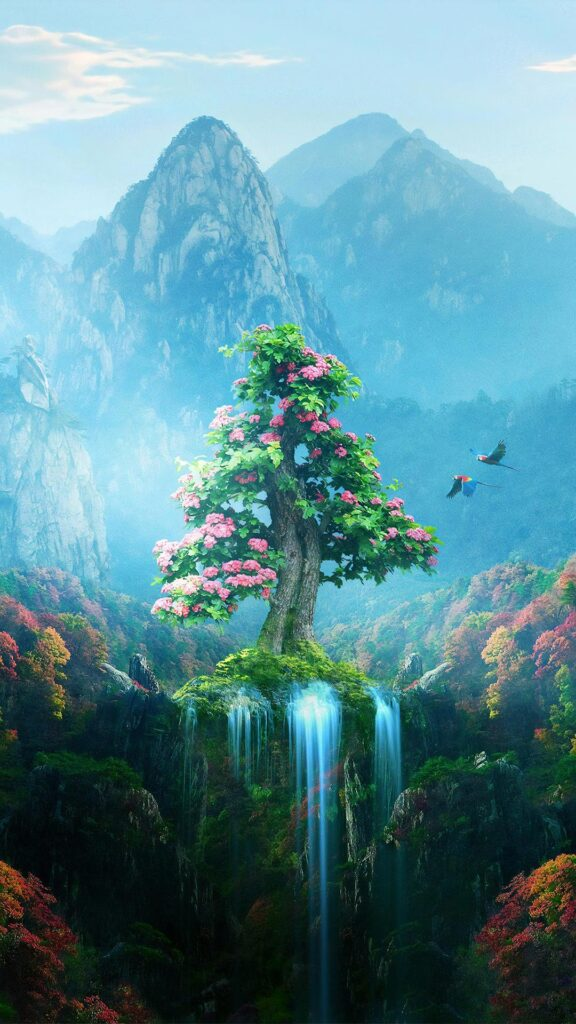
\includegraphics[height=3cm]{example_images/nature2-576x1024.jpg}};
            \end{tikzpicture}
        \end{center} 
    \end{frame}

    \section{Equations}
    \begin{frame}{Frame in ninth section}
        \begin{equation}
            \text{RM} = \int n_e B_{\parallel}\,dl
        \end{equation}
    \end{frame}

    

\end{document}
